\documentclass[11pt]{article}
\usepackage[round]{natbib}
\usepackage{graphicx}
\usepackage{listings}
\usepackage{caption}
\usepackage{subcaption}
\usepackage{pgf}
\usepackage[margin=1in]{geometry}

\begin{document}

\title{On the Performance of String Search Algorithms for Deep Packet Inspection}
\author{Kieran Hunt}
\date{\today}
\maketitle

\section{Introduction}

In Deep Packet Inspection today, systems are generally built on top of expensive custom hardware. Making changes to such a system (such as horizontally scaling) is often arduous, time consuming and expensive. Deep Packet Inspection via software means is usually slower but does provide some benefit: adding or removing capacity to perform inspection is often as simple as adding or removing hosts doing the inspection. String search algorithms have long been of interest to the field of computer science and as a result a substantial number of search algorithms exist. This paper looks to ask which of these string search algorithms perform best at deep packet inspection and how does their performance compare to that of their intended design.

Relevant Deep Packet Inspection terminology is as follows:
\begin{itemize}
  \item \textbf{Packet}: Data representing a TCP/IP stack packet. This includes information from the network to the application layer.
  \item \textbf{Packet Capture File (PCAP)}: A file containing packets. These packets were generally captured by recording a network interface.
  \item \textbf{Deep Packet Inspection (DPI)}: the process by which a packet, or stream of packets, is analysed for the presence of predefined patterns.
\end{itemize}

In order to properly test these string search algorithms, a system was designed to accurately compare each algorithm for inspection of both packet captures as well as textual inputs such as text files.

In the system for comparing string search algorithms, the following terminology is relevant:
\begin{itemize}
  \item \textbf{Input}: This is the interface through which the system reads in either the packets or textual Input. Algorithms can request a single byte from the input, the length of the Input or the entire Input itself.
  \item \textbf{Rule}: The system searches through the input for a given Rule. Rules are very similar to input in that a single byte of information, the length of the rule or the entire rule itself can be requested. 
  \item \textbf{Algorithm}: This represents a string search algorithm and is the means by which the system interacts with all of the algorithms. It has a single interface for performing a search where the Input is supplied and a Result is returned.
  \item \textbf{Result}: This represents the result of the inspection of a single Input. In it is the start and end times of the inspection, the Rules, Input and the location (if any) in the Input where the Rules were matched.
\end{itemize}

Each of the string search algorithms have known performance (algorithm complexity known as big O) usually related to the length of the string being searched. The results of the following experiments should follow the predicted complexity of string search algorithms. Algorithm complexity often only provides insight into large variations in Input length (differing orders of magnitude) whereas in packet data has a limited range of Input lengths and so it may come down to minutiae within the algorithms themselves rather than their overall complexity.

\section{String Search Algorithms}

A vast collection of string search algorithms has been amassed by \citet{charras2004} and from that a selection of algorithms was chosen to implement, benchmark and then compare.
Table \ref{table-algorithms} has a list of each algorithm, the year it was publish, its author(s) and the time complexity of searching with that algorithm.

\begin{table}[!hbt]
\resizebox{\textwidth}{!}{
\begin{tabular}{l|lll}
  Algorithm & Year & Author(s) & Time Complexity \\
  \hline
  Naive & & & O(mn) \\
  MorrisPratt & \citeyear{morris1970} & \citeauthor{morris1970} & O(n + m) \\
  KnuthMorrisPratt & \citeyear{knuth1977} & \citeauthor{knuth1977} & O(n + m) \\
  BoyerMoore & \citeyear{boyer1977} & \citeauthor{boyer1977} & O(nm) \\
  Horspool & \citeyear{horspool1980} & \citeauthor{horspool1980} & O(n + m) \\
  ApostolicoGiancarlo & \citeyear{apostolico1986} & \citeauthor{apostolico1986} & O(n) \\
  RabinKarp & \citeyear{karp1987} & \citeauthor{karp1987} & O(mn) \\
  ZhuTakaoka & \citeyear{feng1987} & \citeauthor{feng1987} & O(mn) \\
  QuickSearch & \citeyear{sunday1990} & \citeauthor{sunday1990} & O(mn) \\
  Smith & \citeyear{smith1991} & \citeauthor{smith1991} & O(mn) \\
  ApostolicoCrochemore & \citeyear{apostolico1991} & \citeauthor{apostolico1991} & O(n) \\
  Colussi & \citeyear{colussi1991} & \citeauthor{colussi1991} & O(n) \\
  Raita & \citeyear{raita1991} & \citeauthor{raita1991} & O(nm) \\
  GalilGiancarlo & \citeyear{galil1991} & \citeauthor{galil1991} & O(n) \\
  Bitap (Shift Or) & \citeyear{baezayates1992} & \citeauthor{baezayates1992} & O(n) \\
  NotSoNaive & \citeyear{hancart1993} & \citeauthor{hancart1993} & O(nm) \\
  Simon & \citeyear{simon1994} & \citeauthor{simon1994} & O(n + m) \\
  TurboBoyerMoore & \citeyear{crochemore1994} & \citeauthor{crochemore1994} & O(n) \\
  ReverseColussi & \citeyear{colussi1994} & \citeauthor{colussi1994} & O(n)
\end{tabular}}
\caption{Implemented string search algorithms for the purpose of comparison against a packet dataset. Under time complexity, \textit{n} represents the length of the Input and \textit{m} represents the length of a Rule. The time complexity is multiplied by a factor equal to the number of Rules.}
\label{table-algorithms}
\end{table}

The time complexities in Table \ref{table-algorithms} should only serve as a basic indication of the speed of an algorithm. Big-O notations generally strip off any factors and so two algorithms may appear to have the same time complexities but in practice their speeds differ greatly because of this unknown factor.

Another point to note is that because these algorithms were designed to search for a single Rule, their Big-O notations only reflect that property. For multiple rules, and a serial-style approach, these algorithms need to run back-to-back; this increases increases their time to process by a factor equal to the number of Rules. For a parallel-style approach searches for different rules using the same algorithm can be run at the same time. The speed at which a search for a complete set of Rules completes is then both related to the algorithmic complexity of the search as well as the number of rules which are being searched for at the same time.

An upper bound for the number of concurrent searches for different Rules with the same Algorithm and Input exists. That upper bound is defined by the number of processor cores that are available for use.

\section{Method}

As mentioned previously, a system was developed to allow accurate running and performance measurement of each of the implemented algorithms (in Table \ref{table-algorithms}). The system takes a json file as input (See Listing \ref{listing-testConfiguration.json}). For the test, the following configuration was chosen:
\begin{itemize}
  \item \texttt{algorithms} - a list of all implemented Algorithms (See Table \ref{table-algorithms}) 
  \item \texttt{rules} - string-based rules covering the twenty most popular websites \citep{alexa2016} - just their domain names were taken - as well as the twenty most popular words in the English language \citep{oed2016}.
  \item \texttt{inputs} - a dataset of DNS traffic was selected and a subset of 10000 packets was extracted. This was labeled \texttt{smallcapture.pcap}. A second Input was also selected, this is the complete \textit{Alice in Wonderland} by Lewis Carol. This Input was labeled \texttt{alice.txt}. The system treats text and pcap input files differently. Text input files are used to create a single Input object representing all information in that file. Pcap input files are split up into individual packet objects and each packet represents a single Input.
  \item \texttt{times} - the tests were each run 20 times.
  \item \texttt{threadCount} - drastic speed increases are made possible by splitting the work of the Algorithms across multiple threads. The machine used to perform the test has 24 useable cores and so a max \texttt{threadCount} of 18 was chosen to best make use of those cores.
\end{itemize}


\begin{lstlisting}[caption = {Sample testConfiguration.json}, label = {listing-testConfiguration.json}]
{
  "algorithms": [
    "Naive",
    "MorrisPratt",
    ...
    "ReverseColussi"
  ],
  "rules": [
    "time",
    "person",
    ...
    "msn"
  ],
  "inputs": [
    {
      "type": "pcap",
      "location": "smallcapture.pcap"
    },
    {
      "type": "text",
      "location": "alice.txt"
    }
  ],
  "times": 20,
  "threadCount": 18
}
\end{lstlisting}

\begin{table}[hbt]
  \centering
  \begin{tabular}{cccccc}
    Minimum & First Quartile & Median & Mean & Third Quartile & Maximum \\
    \hline
    54.0 & 81.0 & 85.0 & 109.8 & 99.0 & 585.0
  \end{tabular}
  \caption{\textit{Dataset A} packet length statistics.}
  \label{table-inputsummary}
\end{table}


\section{Results}

The test generated 3400340 result objects. Each result object looked very similar to Listing \ref{listing-testresult}. Containing information about the start and end times (in nanoseconds), the elapsed time (the end time - the start time), the rules searched for, the locations that rules were matched at, the algorithm used, the input file, the Input ID, the run number and the ID of that run.

\begin{lstlisting}[caption = {Sample test Result}, label = {listing-testresult}]
[
    {
        "start": 206079193307938,
        "end": 206079207132342,
        "elapsed": 13824404,
        "rules": [
            "time",
            "person",
            ...
            "msn"
        ],
        "locations": [1, 2, ..., n],
        "algorithm": "Smith",
        "inputFile": "smallcapture.pcap",
        "inputID": "bf75faa5",
        "runNumber": 1,
        "runId": "d9b4a28aefbd"
    },
    ...
]
\end{lstlisting}

\section{Analysis}

\subsection{Which Algorithms are Fastest? Which are Slowest?}

Figure \ref{figure-barmeanprocessingsmallcapture} shows a comparison of processing times for each algorithm over each of the packets in PCAP dataset. Figure \ref{figure-barmeanprocessingalice} gives the same comparison albeit for the \textit{Alice in Wonderland} input file.

\begin{figure}[t]
    \centering
    \begin{subfigure}[b]{\textwidth}
        \centering
        \includegraphics[width=0.85\textwidth]{images/bar_graph_mean_one_input_smallcapture_pcap}
        \label{figure-barmeanprocessingsmallcapture}
        \caption{Mean Input processing times of each Algorithm for \textit{PCAP Dataset}.}
    \end{subfigure}
    ~
    \begin{subfigure}[b]{\textwidth}
        \centering
        \includegraphics[width=0.85\textwidth]{images/bar_graph_mean_one_input_alice_txt}
        \label{figure-barmeanprocessingalice}
        \caption{Mean Input processing times of each Algorithm for \textit{Alice in Wonderland}.}
    \end{subfigure}
    \caption{Mean input processing times for each algorithm.}
\end{figure}

Taking into account the processing speed of each algorithm from both Figure \ref{figure-barmeanprocessingsmallcapture} and \ref{figure-barmeanprocessingalice} we are able to list the algorithms in order of their processing speed - fastest first: Horspool, Quicksearch, Raita, ReverseColussi, BoyerMoore, ZhuTakaoka, Smith, Colussi, KnuthMorrisPratt, TurboBoyerMoore, ApostolicoGiancarlo, MorrisPratt, Naive, Simon, Bitap, NotSoNaive, RabinKarp. 

Although the order of speediness changes between Figure \ref{figure-barmeanprocessingsmallcapture} and \ref{figure-barmeanprocessingalice}, the position of the algorithms varies by less than four places.

The relative speed difference of each algorithm in Figure \ref{figure-barmeanprocessingsmallcapture} appears to be quite small. By increasing the length of the input data (in this case by using the \textit{Alice in Wonderland} text. Figure \ref{figure-barmeanprocessingalice}) we are able to accentuate the differences. 

\begin{table}[hbt]
  \centering
  \resizebox{\textwidth}{!}{
  \begin{tabular}{l|cccccc}
    Algorithm & Minimum & First Quartile & Median & Mean & Third Quartile & Max \\
    \hline
    QuickSearch & 0.08321 & 0.10750 & 0.11430 & 0.16350 & 0.12320 & 259.70000 \\
    Horspool & 0.0926 & 0.1098 & 0.1166 & 0.1640 & 0.1246 & 5.3770 \\
    ReverseColussi & 0.09139 & 0.11180 & 0.11910 & 0.16410 & 0.12740 & 5.70000 \\
    Raita & 0.09035 & 0.10710 & 0.11600 & 0.16560 & 0.12440 & 164.10000 \\
    ZhuTakaoka & 0.09288 & 0.11200 & 0.11900 & 0.16560 & 0.12740 & 4.64500 \\
    KnuthMorrisPratt & 0.09113 & 0.11180 & 0.11930 & 0.16630 & 0.12780 & 25.96000 \\
    Colussi & 0.09178 & 0.11130 & 0.11840 & 0.16640 & 0.12670 & 29.69000 \\
    Smith & 0.09102 & 0.11170 & 0.11880 & 0.16710 & 0.12660 & 5.33400 \\
    BoyerMoore & 0.09287 & 0.11070 & 0.11740 & 0.16730 & 0.12540 & 33.22000 \\
    MorrisPratt & 0.08543 & 0.10910 & 0.11540 & 0.16750 & 0.12360 & 297.80000 \\
    Naive & 0.08845 & 0.11180 & 0.11830 & 0.16820 & 0.12620 & 63.84000 \\
    Bitap & 0.09277 & 0.11160 & 0.11900 & 0.16840 & 0.12780 & 50.14000 \\
    TurboBoyerMoore & 0.09101 & 0.11220 & 0.11900 & 0.16880 & 0.12680 & 41.68000 \\
    RabinKarp & 0.09562 & 0.11580 & 0.12230 & 0.17070 & 0.13200 & 245.60000 \\
    Simon & 0.08248 & 0.11140 & 0.11890 & 0.17320 & 0.12750 & 117.20000 \\
    ApostolicoGiancarlo & 0.09368 & 0.11420 & 0.12170 & 0.17340 & 0.13020 & 5.06700 \\
    NotSoNaive & 0.1092 & 0.1698 & 0.2277 & 0.3806 & 0.2957 & 552.3000 \\
  \end{tabular}}
  \caption{Algorithm processing speed summary for \textit{Dataset A}}
  \label{table-algorithmspeed}
\end{table}

The \textit{slowest} algorithms were NotSoNaive and RabinKarp.

RabinKarp's \citep{karp1987} slowness can easily be attributed to both its O(mn) complexity as well as its constant recalculation of the input hash. 
NotSoNaive's \citep{hancart1993} slowness is surprising at first. It performs worse than the Naive algorithm when it is supposed to be an improvement on it. The NotSoNaive algorithm tries to improve upon the Naive algorithm by adding a adding a check to see if the Input ahead shows signs of matching the Rule; this extra step seems to cause the speed decrease when compared to Naive. By checking \ref{table-algorithmspeed}, you may think that the mean processing time for NotSoNaive was heavily influenced by the maximum speed (that is to say that that value is an outlier) but by checking the median processing it is clear that the mean is not far from it.

The \textit{fastest} algorithms were QuickSearch and Horspool.

QuickSearch \citep{sunday1990} makes use of the BoyerMoore \citep{boyer1977} algorithm's bad-character shift table. The algorithm is known to perform well for short rule \citep{leqroc1995} and since rules used in the experiment were mostly short, it performed well.
The Horspool \citep{horspool1980} algorithm also makes use of the bad-character shift table from BoyerMoore \citep{boyer1977}. Although the algorithm has a O(mn) complexity, it can be shown that the average number of comparisons made with a character in the Input is $\alpha$, where $\frac{1}{c} \leq \alpha \leq \frac{2}{c+1}$ and $c$ is the number number of characters in the alphabet \citep{baezayates1992b}. In our case our alphabet is 256 characters long (the size of one byte) and so the average number of comparisons to a character in our text is $\frac{1}{256} \leq \alpha \leq \frac{2}{257}$. That is a very low number of comparisons per input character.

\subsection{Do Some Algorithms Perform Differently Depending on the Input Length?}

Figure \ref{figure-speedvslength} shows a scatter plot of Input processing speed versus packet length. This scatter plot shows processing times for all algorithms. Note that the vertical axis has been plotted with a logarithmic scale. From the plot it is clear that there is an upward trend of processing time as the input length increases.

\begin{figure}[t]
    \centering
    \includegraphics[width=0.85\textwidth]{images/scatter_mean_time_vs_input_length_pcap}
    \caption{Input processing speeds vs input length for \textit{Dataset A}.}
    \label{figure-speedvslength}
\end{figure}

\begin{figure}
  \centering
  \begin{subfigure}[b]{0.45\textwidth}
      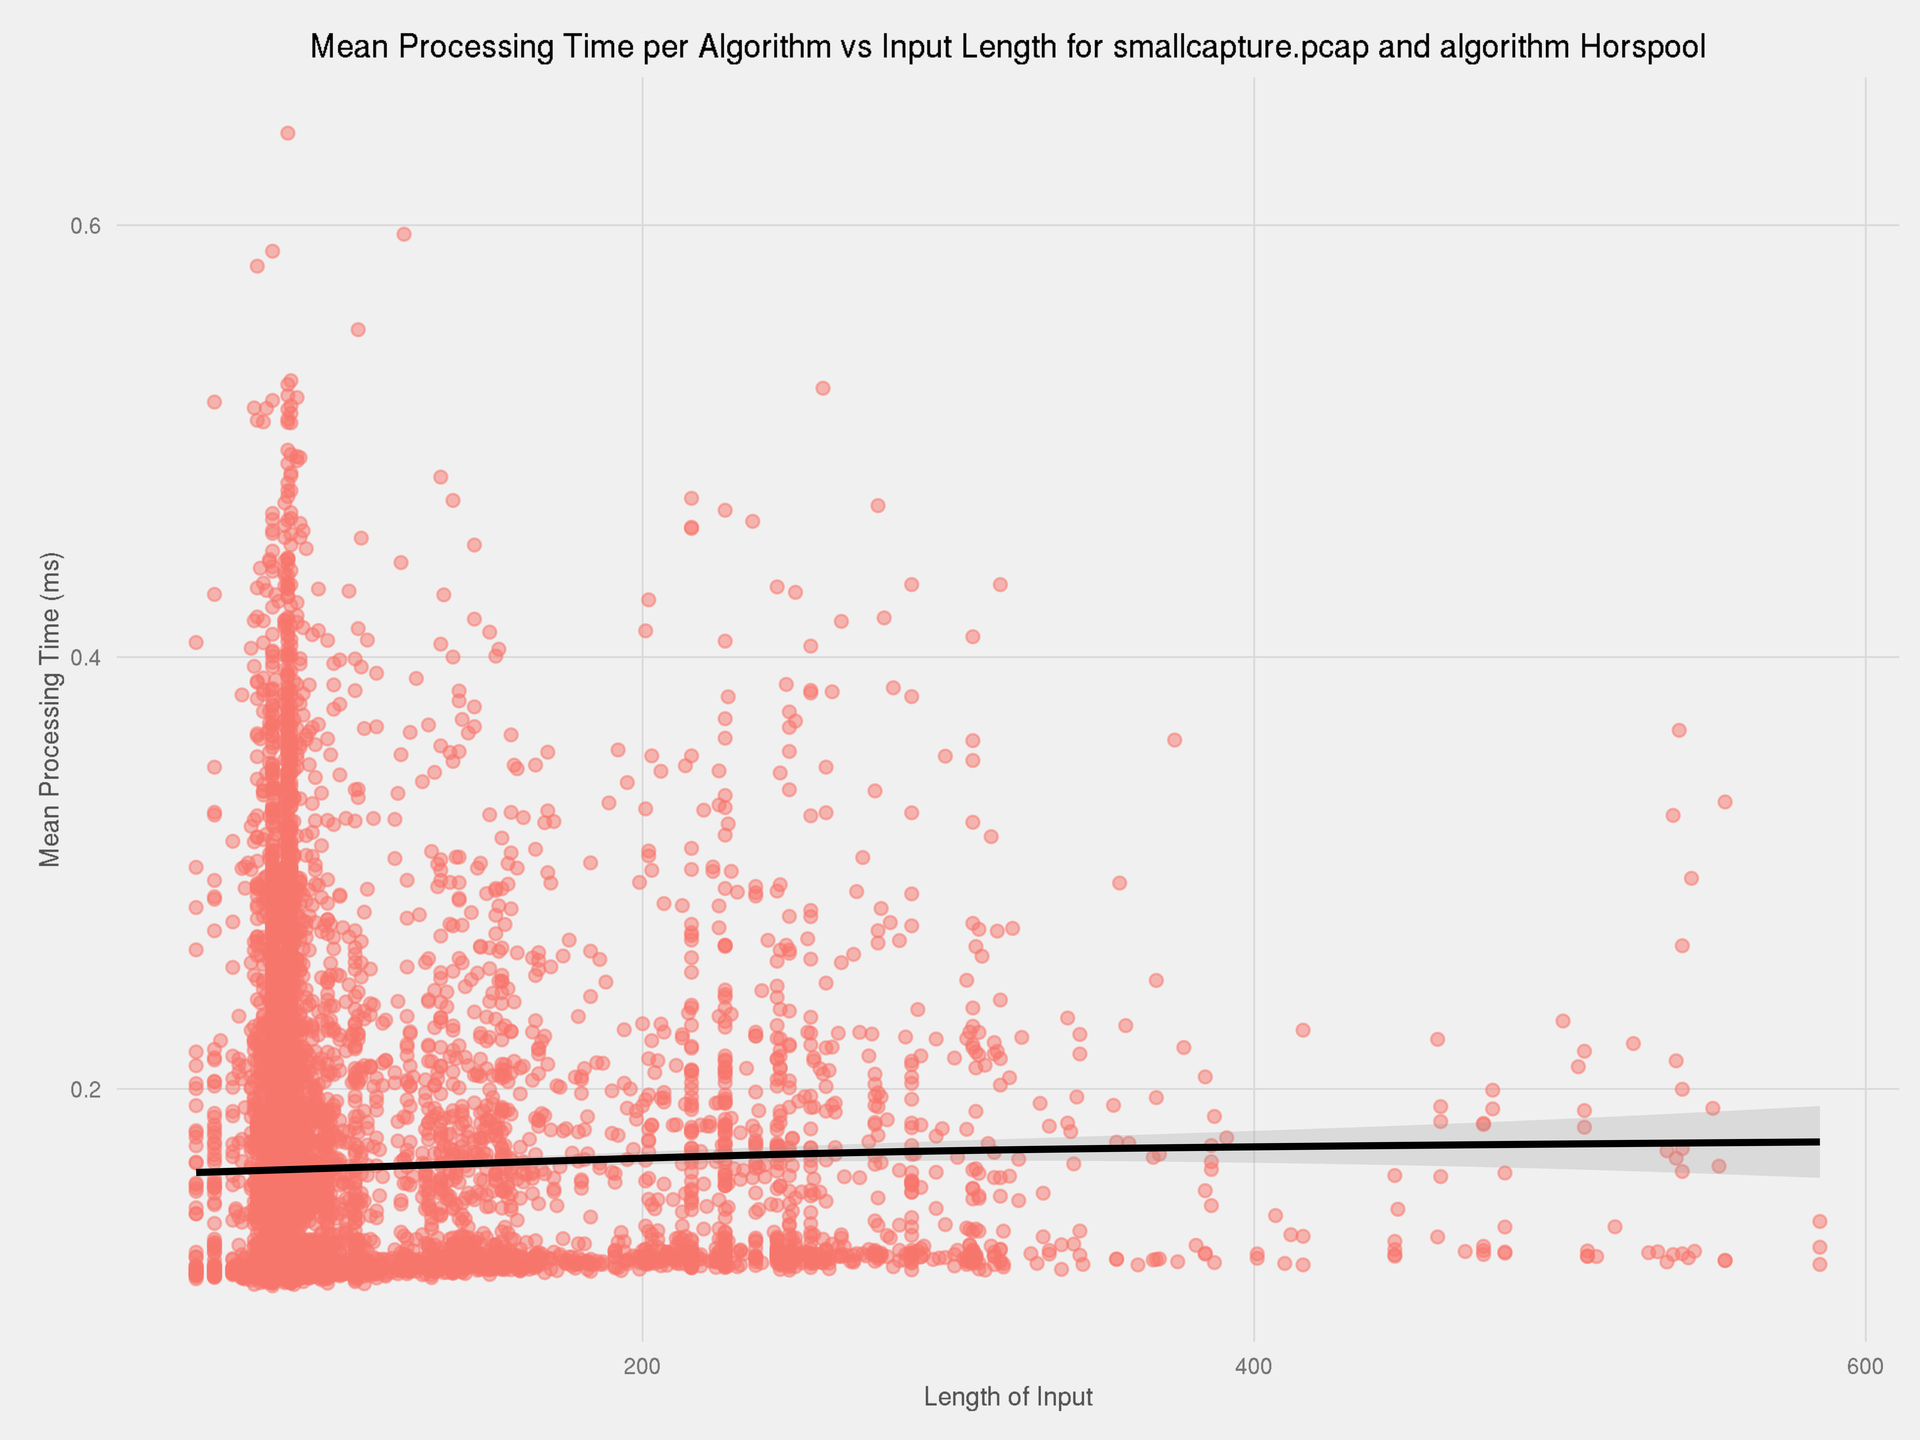
\includegraphics[width=\textwidth]{images/scatter_mean_vs_input_length_Horspool}
  \end{subfigure}
  \begin{subfigure}[b]{0.45\textwidth}
      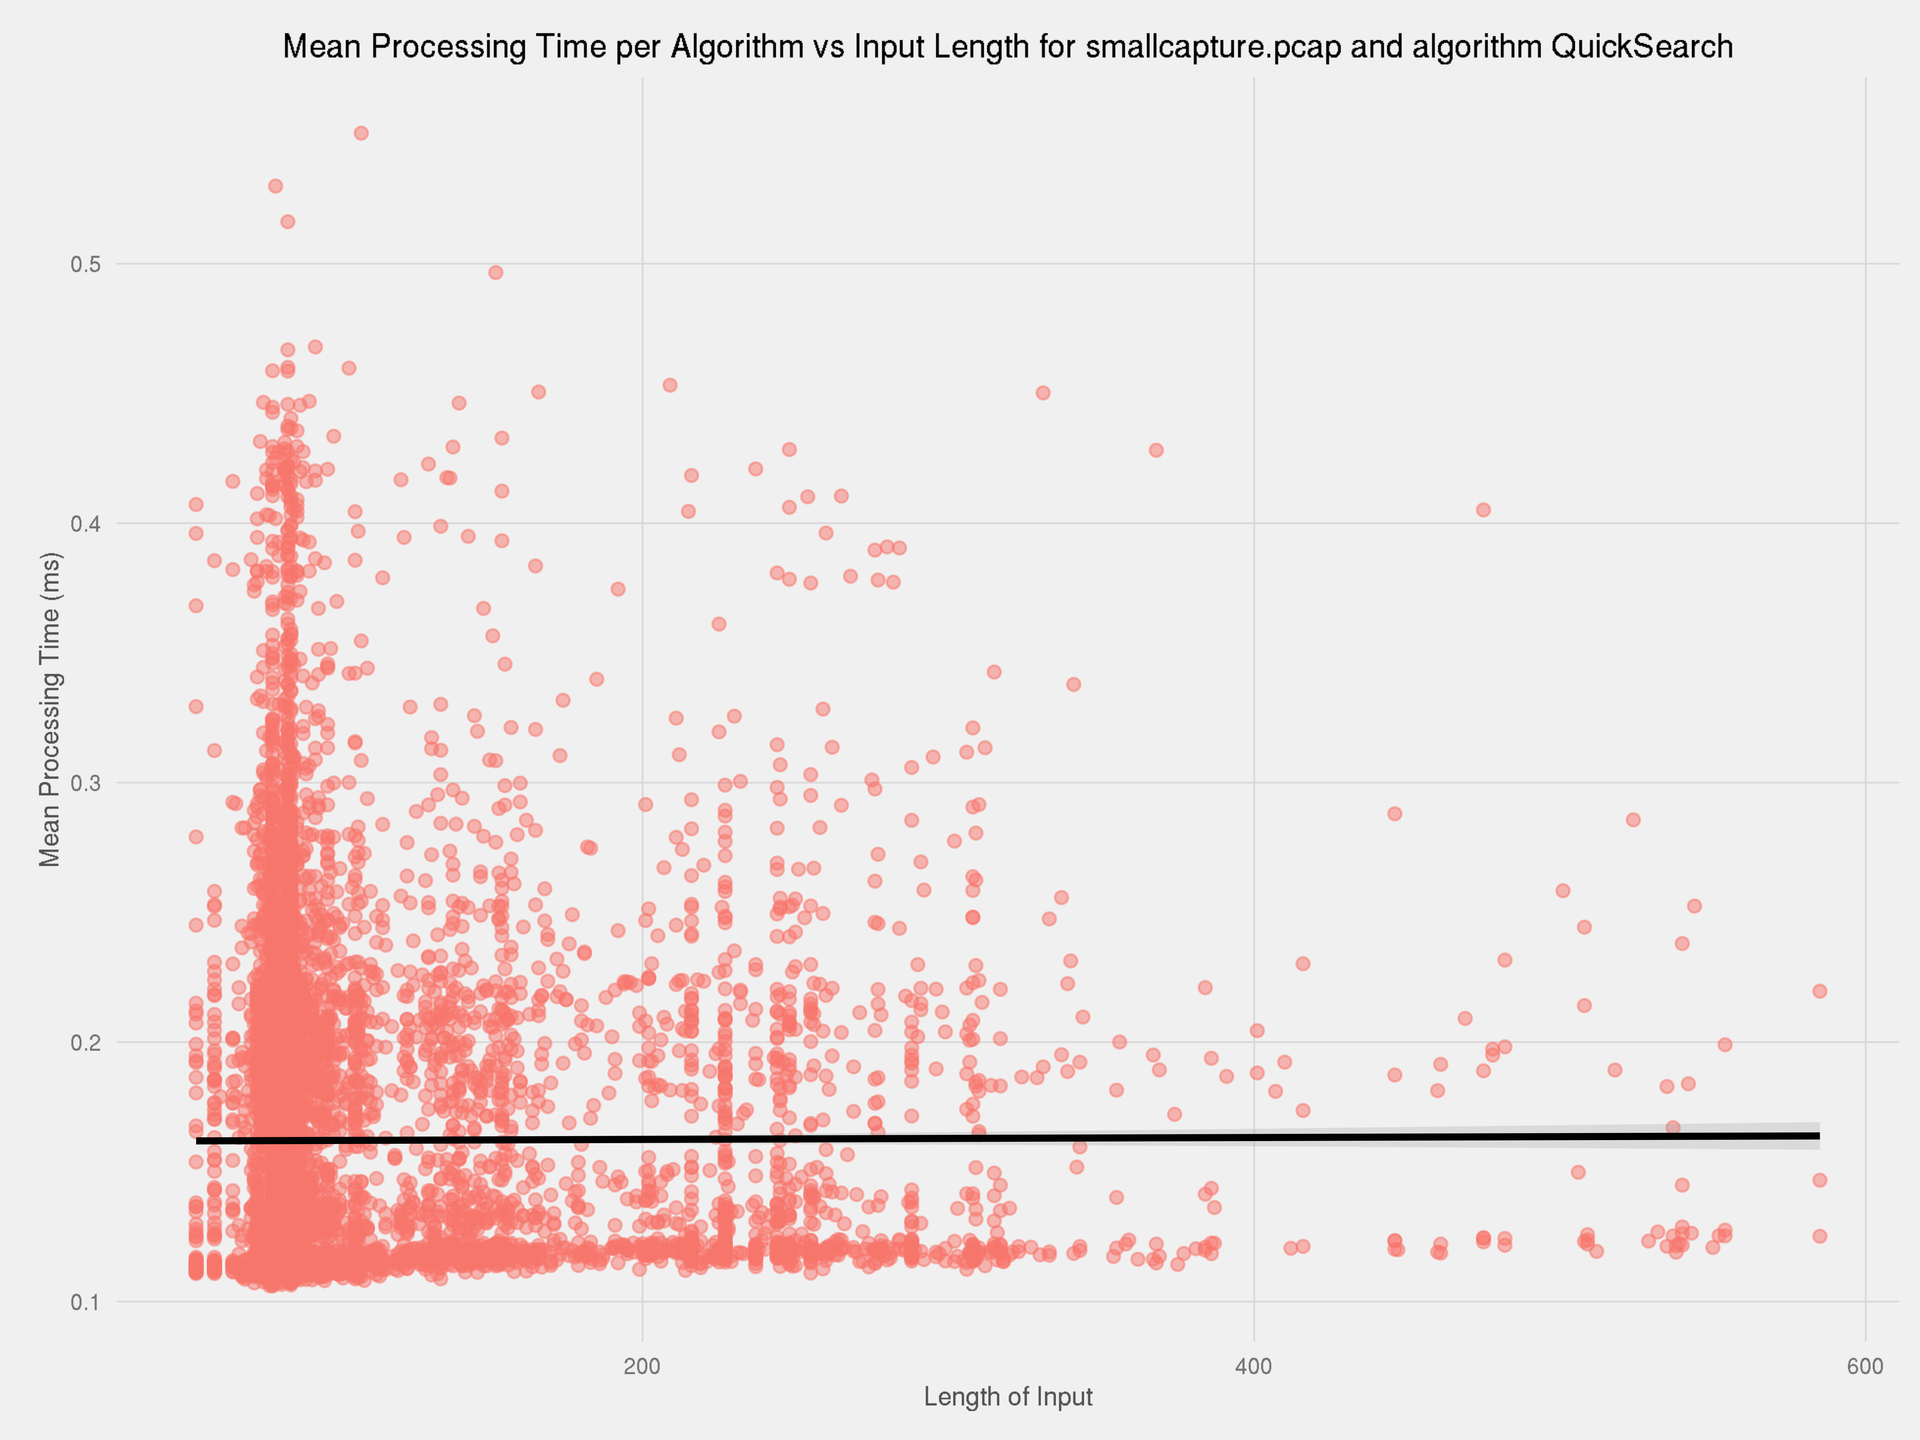
\includegraphics[width=\textwidth]{images/scatter_mean_vs_input_length_QuickSearch}
  \end{subfigure}
  ~
  \begin{subfigure}[b]{0.45\textwidth}
      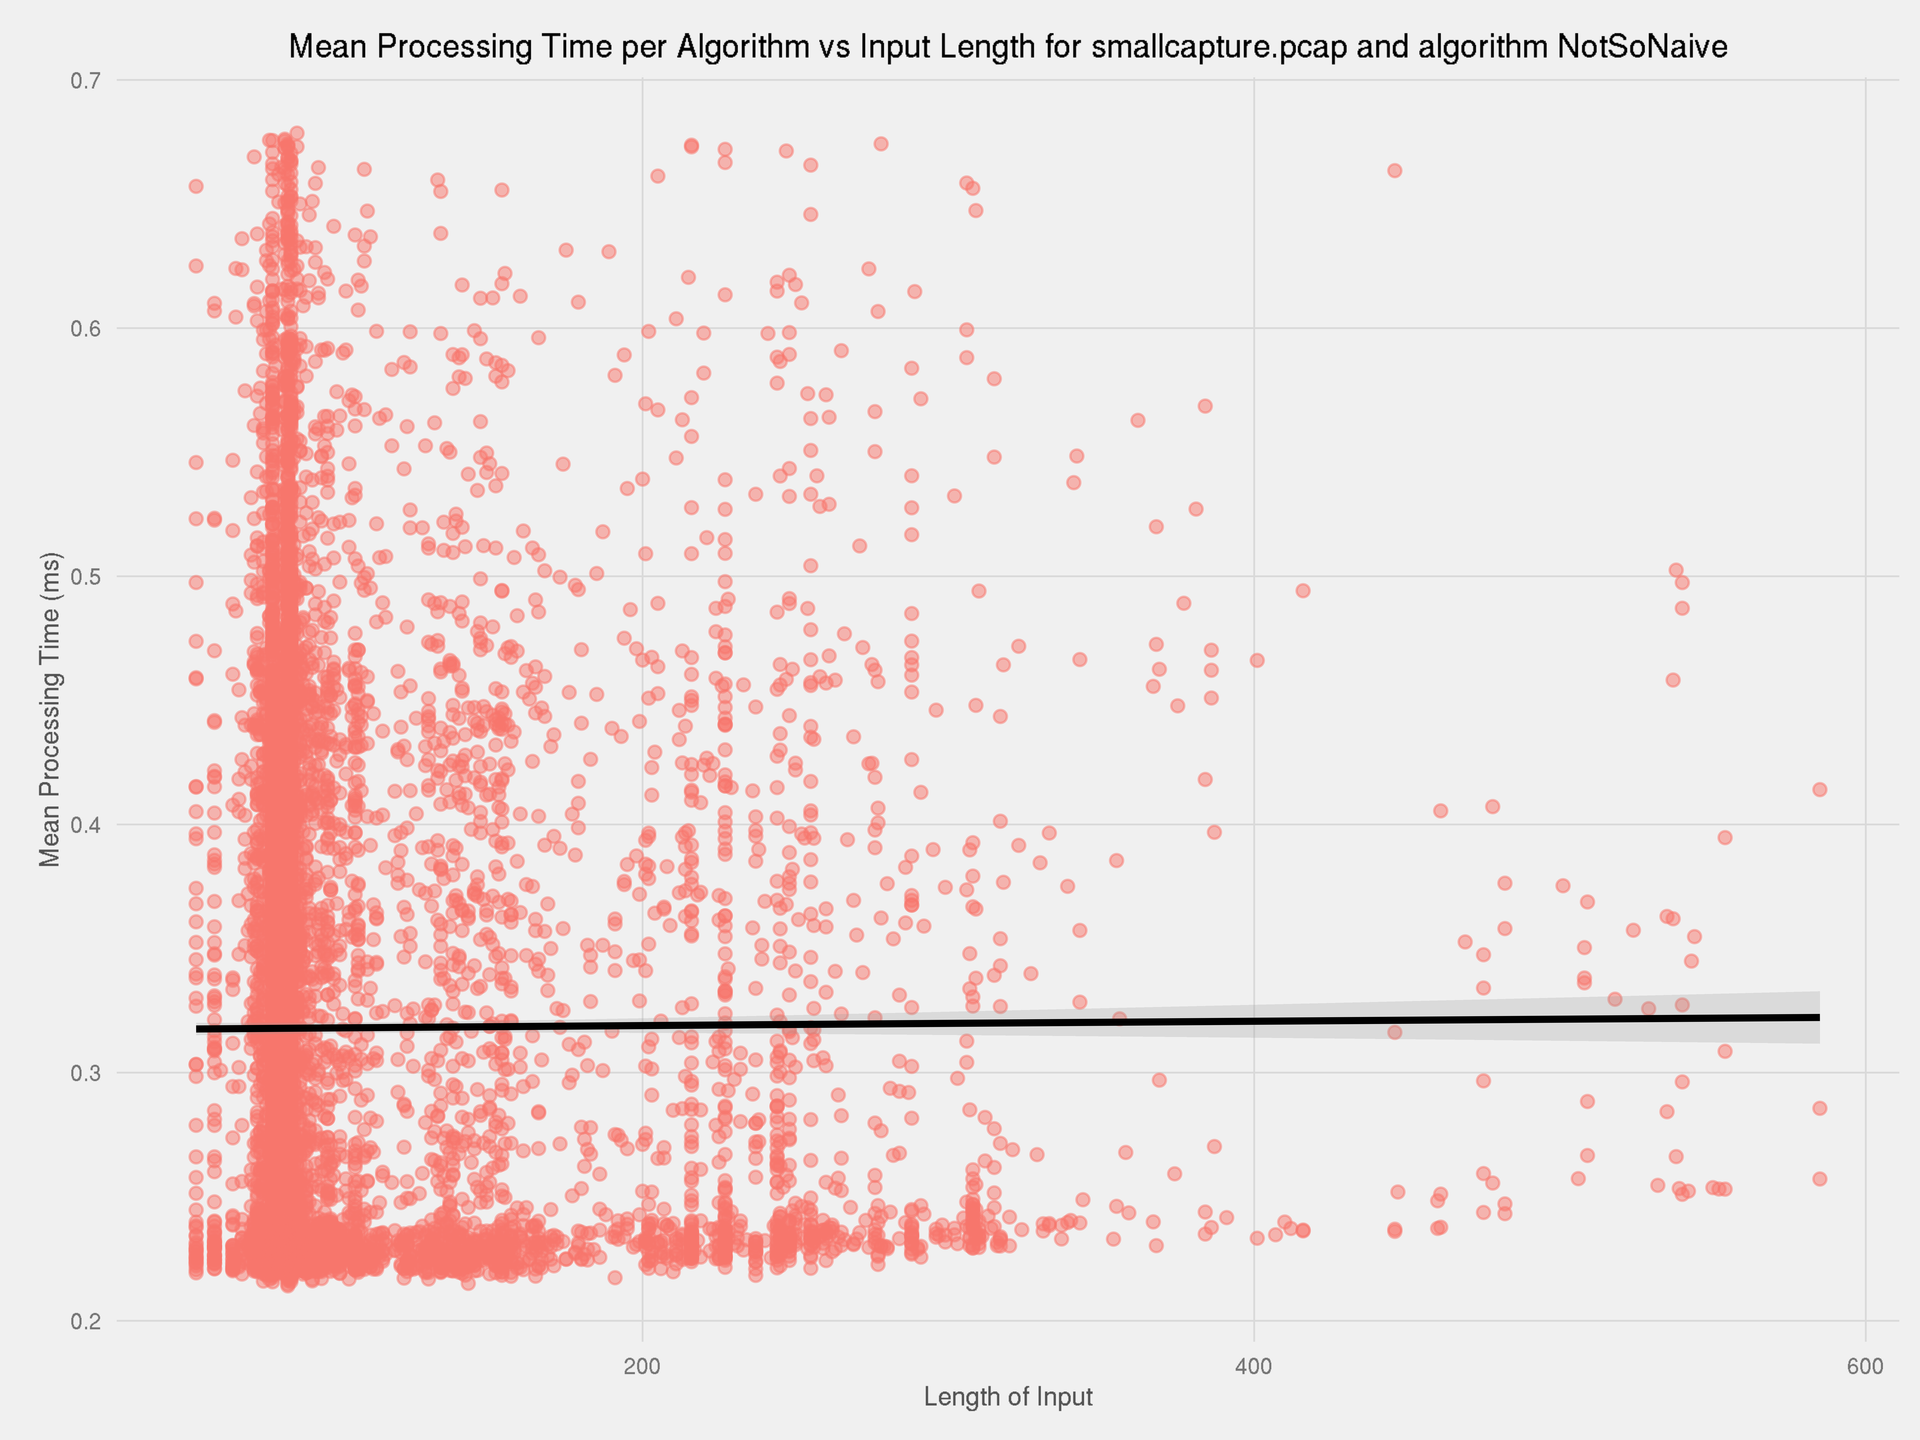
\includegraphics[width=\textwidth]{images/scatter_mean_vs_input_length_NotSoNaive}
  \end{subfigure}
  \begin{subfigure}[b]{0.45\textwidth}
      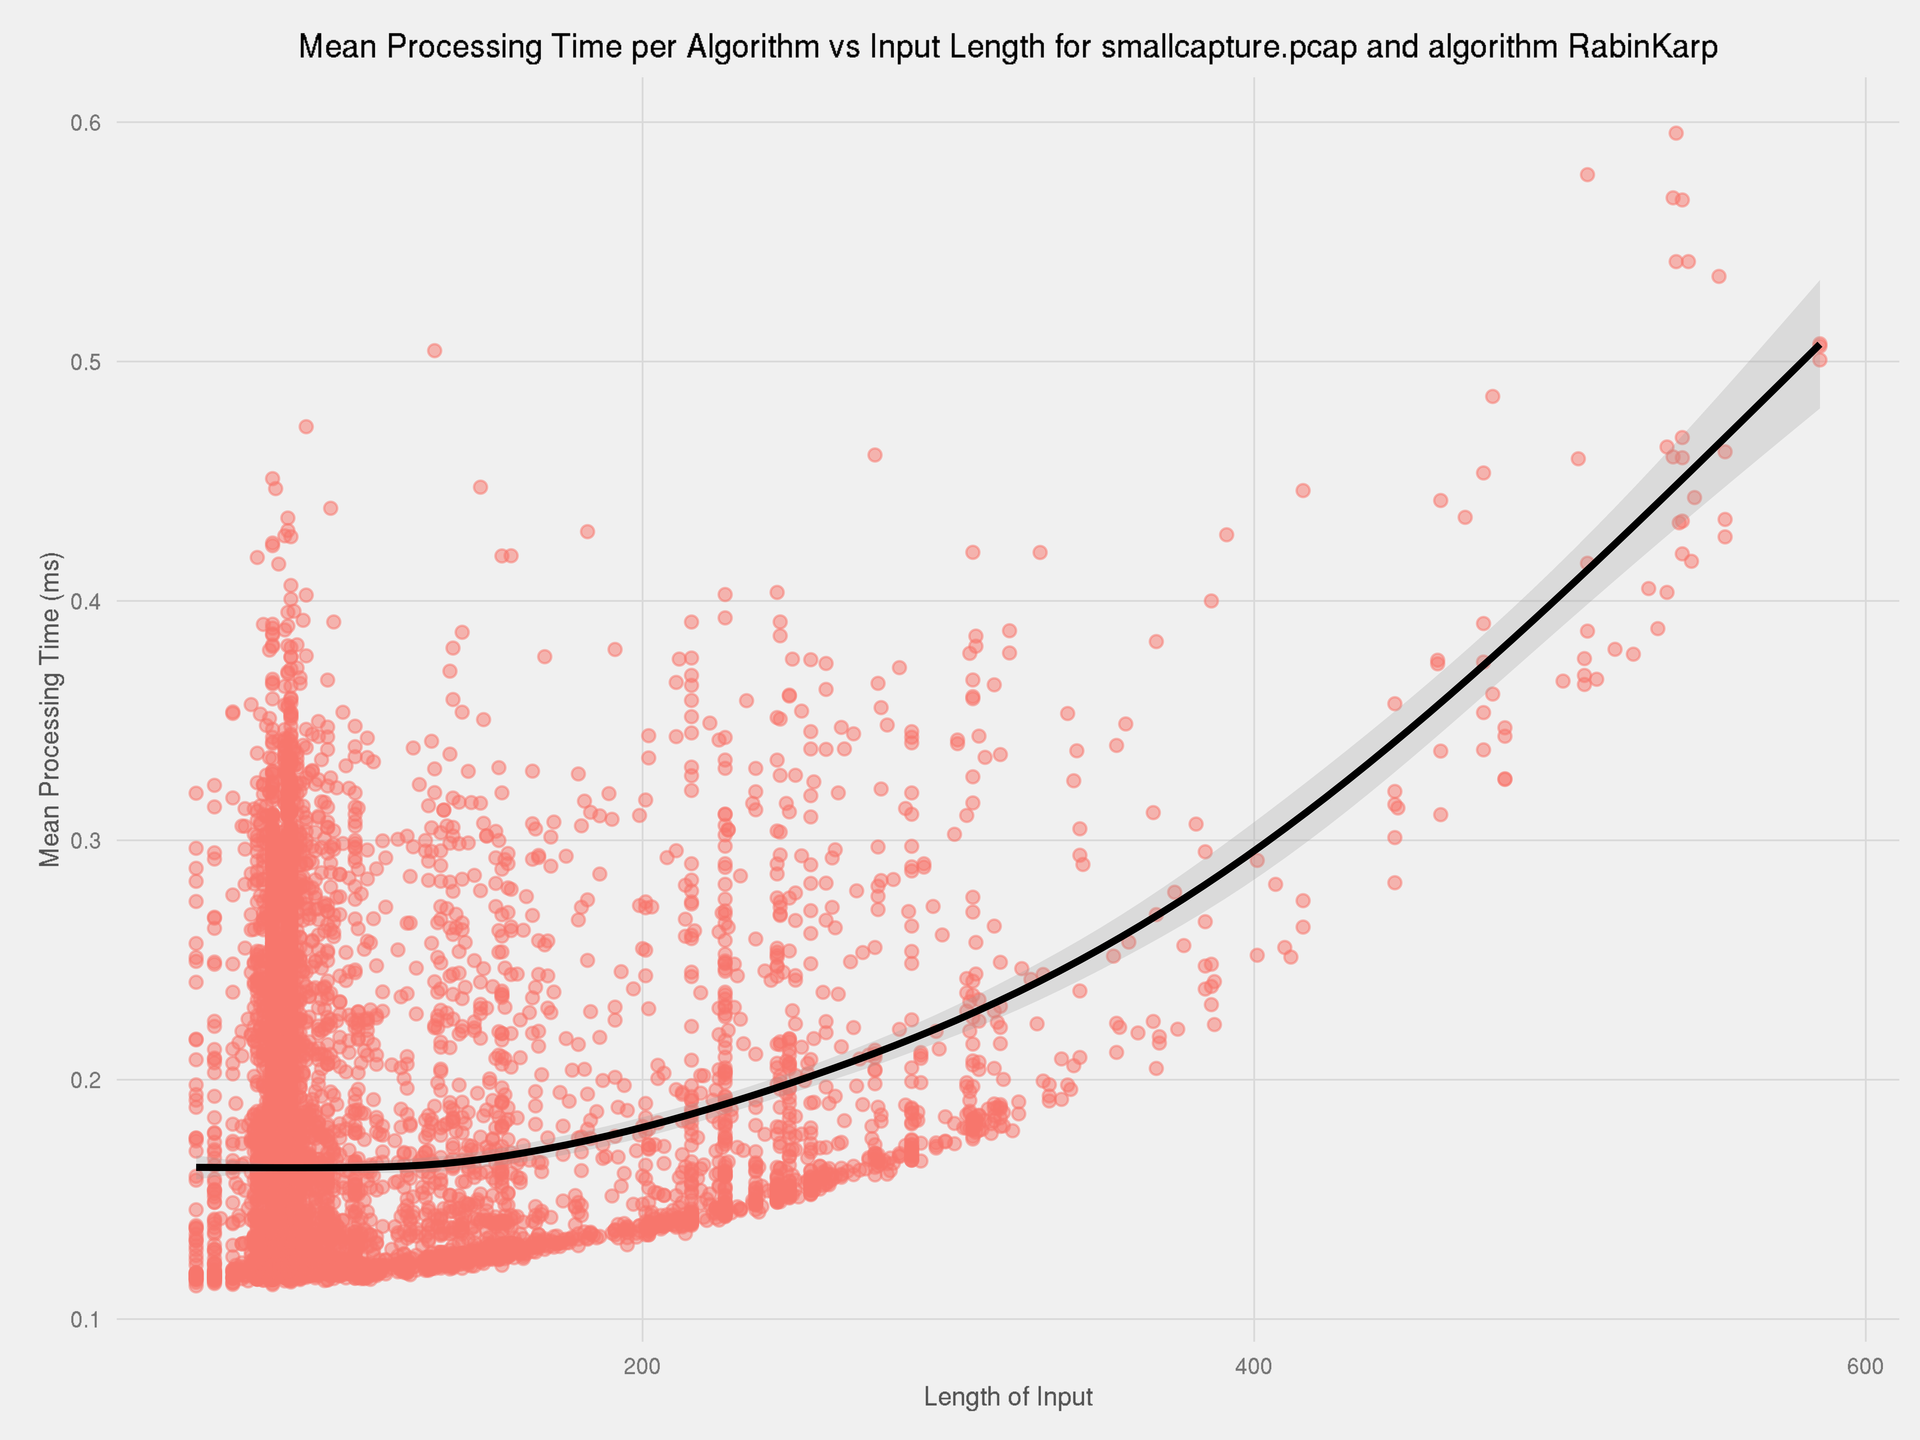
\includegraphics[width=\textwidth]{images/scatter_mean_vs_input_length_RabinKarp}
  \end{subfigure}
  \caption{}
\end{figure}


Algorithms best suited to deep packet inspection would be expected to perform better for smaller input lengths and the performance at input lengths larger than the maximum length of a packet would not matter. Algorithms with a bounded maximum processing time would be especially enticing to a deep packet inspection system implementor as it could guarantee a minimum throughput.

\subsection{Which Algorithms Have the Least Fluctuating Processing Times?}

It is important that algorithms have consistent performance. Algorithms that have highly fluctuating processing speeds lead to unpredictable processing times and unwanted slowdowns of realtime packet inspection.

Figure \ref{figure-standarddeviation} shows the standard deviations of each of the algorithms for \textit{Dataset A}. Most algorithms appear to have relatively low fluctuation on their processing times whilst some are a bit higher. The Horspool \citep{horspool1980} algorithm appears to have a very low standard deviation which, combined with its speed shown in Table \ref{table-algorithmspeed}, makes it a very strong packet processing algorithm.

Another point of interest in Figure \ref{figure-standarddeviation} is that QuickSeach has a notably higher standard deviation than Horspool. It may not be all that well suited to packet inspection as a result.

\begin{figure}[hbt]
  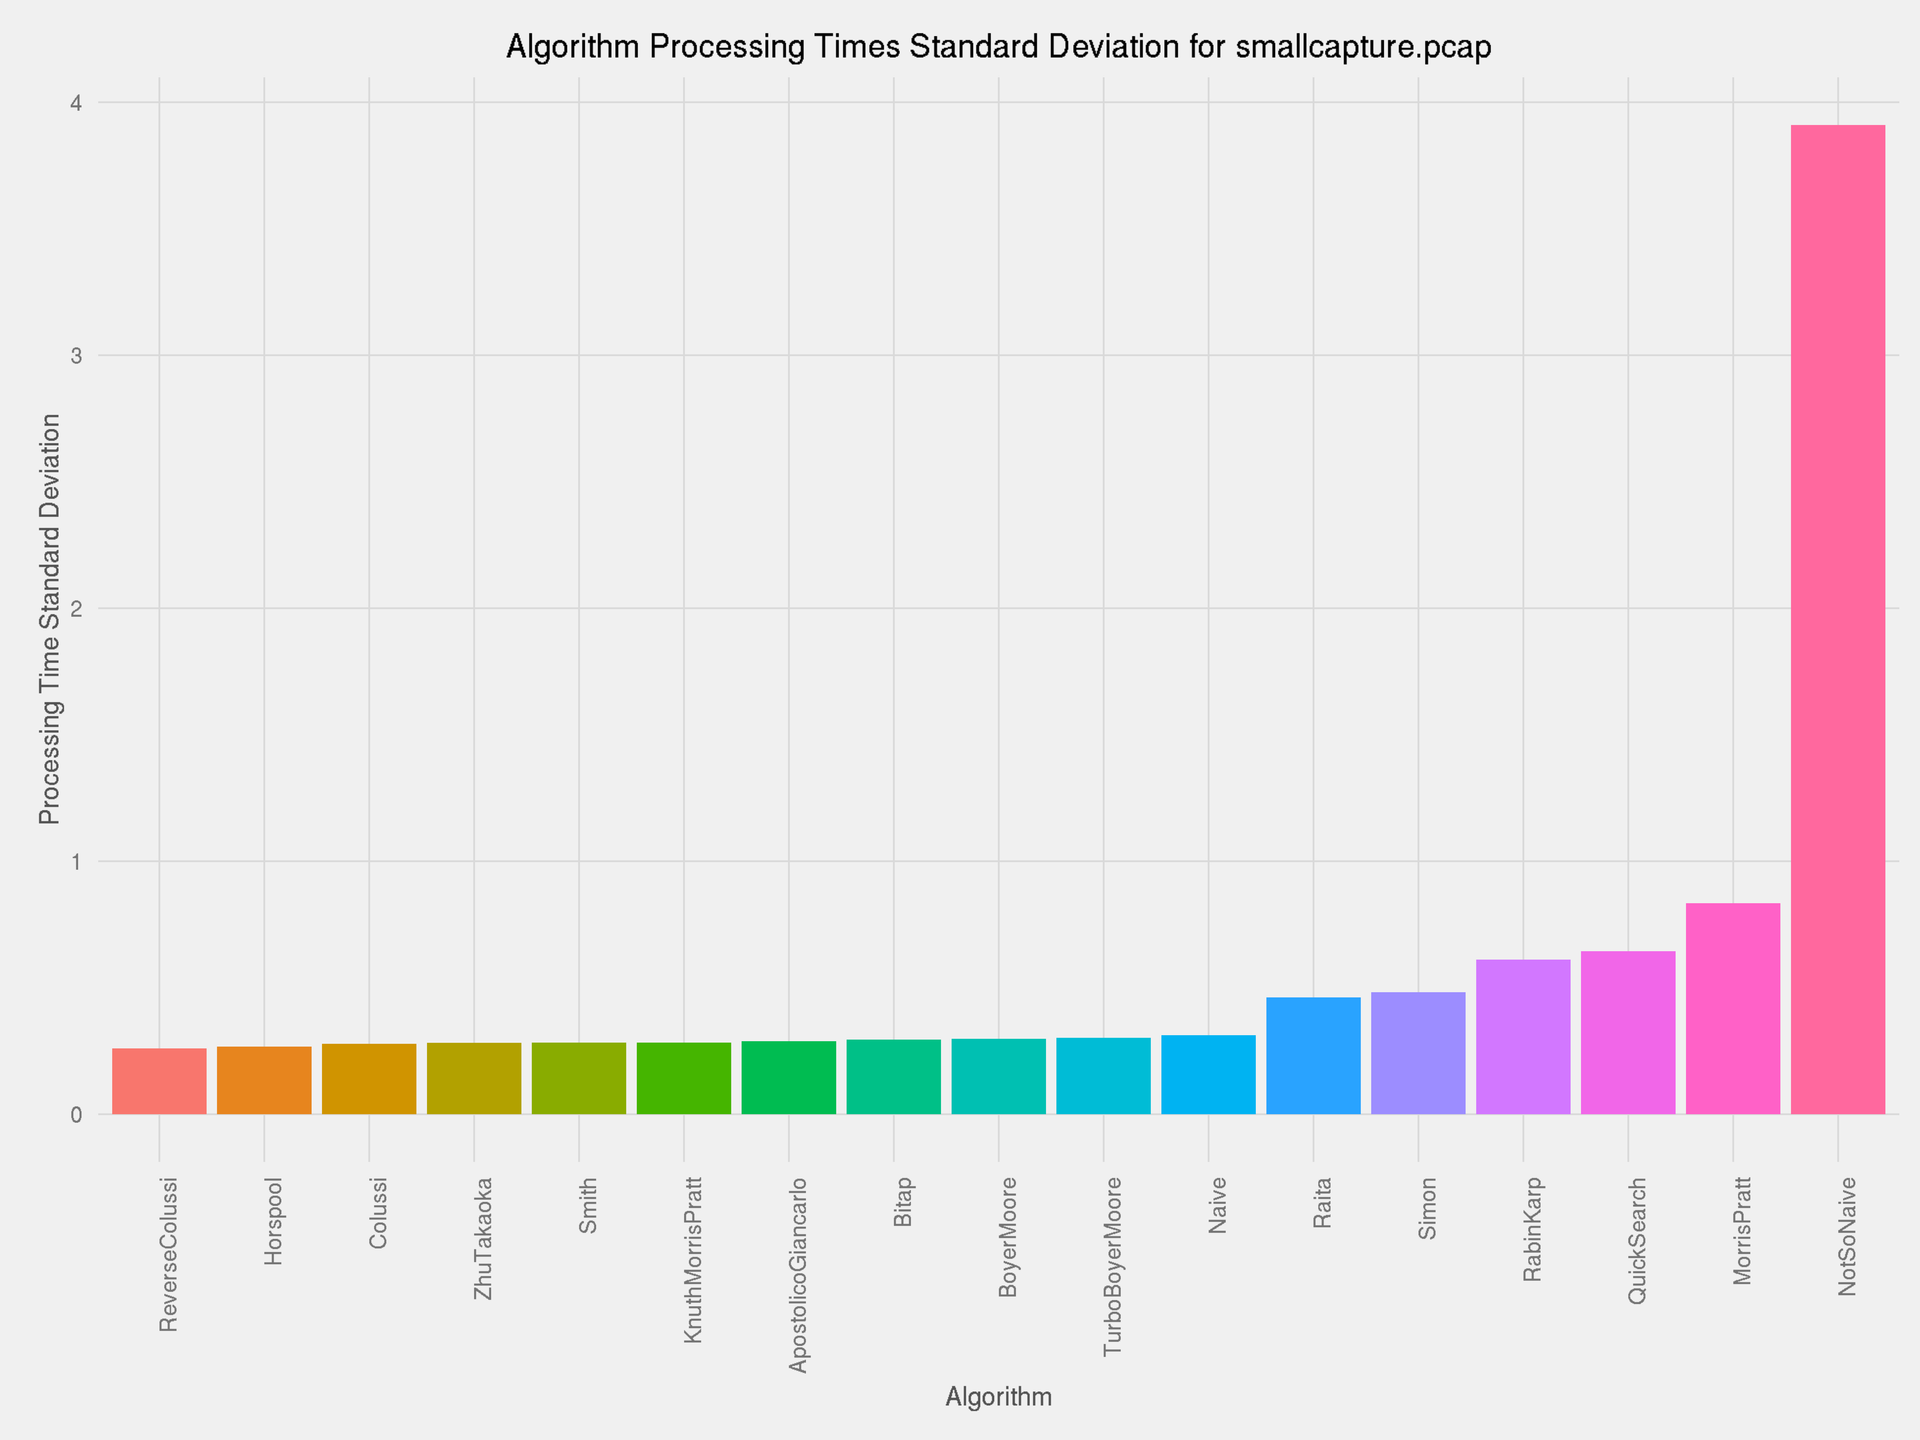
\includegraphics[width=\textwidth]{images/bar_graph_algorithm_standard_deviation_pcap}
  \caption{The standard deviation of processing time per algorithm for \textit{Dataset A}.}
  \label{figure-standarddeviation}
\end{figure}


\subsection{Real World Packet Processing Speeds}

For the packet data, most algorithms have a mean packet processing speed of anywhere between 0.1 and 0.2 milliseconds.

The average processing speed of about 0.15ms (Table \ref{table-algorithmspeed}) as well as an average packet length of about 110 bytes (Table \ref{table-inputsummary}) means that a rough line speed of 6 megabits per second is achievable. This speed is obviously much less than what would be required of a modern Deep Packet Inspection system. The goal of this research is to develop an understand of the algorithms' relative speed.

\section{Conclusion}

Of the original algorithms chosen to test, Horspool \citep{horspool1980} seems to perform best when it comes to packet analysis.
Although software-based deep packet inspection is not as popular as its hardware counterpart, it does provide an easier-to-scale environment that can better cope with the fluctuations of periodic network load.

\bibliographystyle{plainnat}
\bibliography{references}

\end{document}
